\section{Description de la structure}\label{sec:DescStruct}
Avant de commencer à regarder les différentes solutions des points clés du projet il convient de se mettre d'accord
sur la structure principale où tout sera attaché. Cette dernière est faite en profilé Item \cite{Item} comme convenu dans le descriptif
du projet. Le choix de profilé se portera sur le profilé 8 40x40 naturel. Afin de pouvoir le placer sur une table comme demandé, l'installation de pieds sera nécessaire. Les pieds proposé par Item ne
permettent pas une adhérence suffisante à la table et ne sont pas réglables. Elesa \cite{Elesa} possède une grande variété de pieds ce qui
a permis de trouver exactement ce qui était recherché pour ce projet. Le pied GN 6311.6-KR possède une rotule entre le pied
et la vis, un revêtement antiglisse et une vis sans tête M10. Ceux-ci étaient les critères principaux pour le choix des pieds. La fabrication d'une pièce (plan dans les Annexes) pour pouvoir attacher
les pieds au reste de la structure est donc nécessaire. Cette dernière aura un perçage taraudé M10 pour visser un pied et un lamage M8 pour
une vis six pans creux à tête cylindrique qui se fixe sur le côté taraudé des profilés. Voici à quoi ressemble la pièce en question.

\begin{figure}[H]
  \centering
  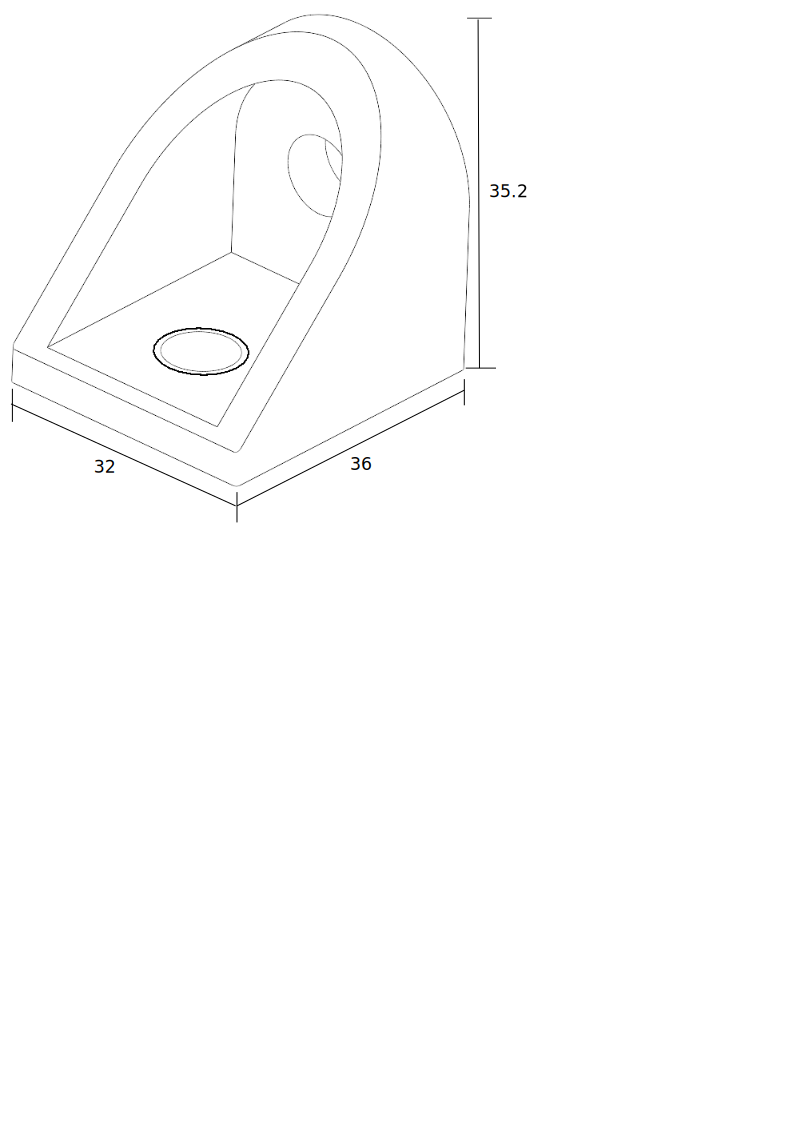
\includegraphics[width = 0.4\textwidth]{assets/figures/SupportPieds.svg}
  \caption{Représentation du support pour les pieds du système}
  \label{fig:SupPieds}
\end{figure}

La structure complète avec les pieds et ses supports ressemble à ceci.
\begin{figure}[H]
  \centering
  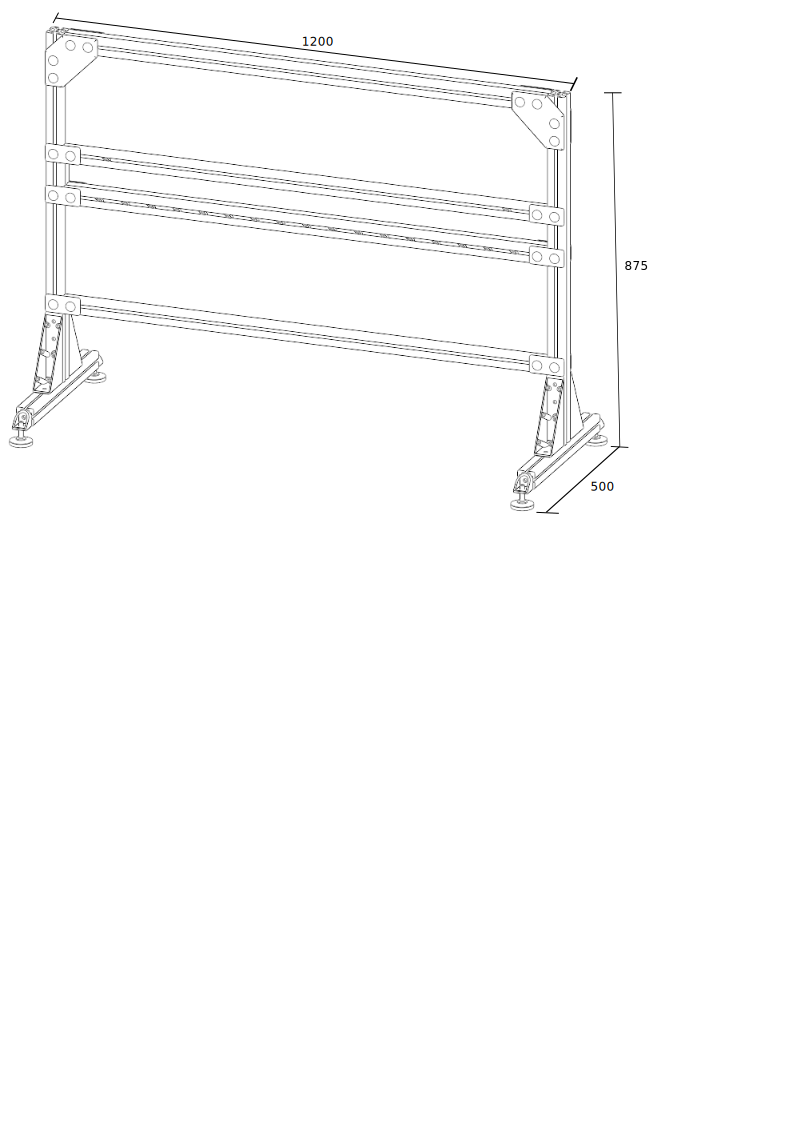
\includegraphics[width = 0.8\textwidth]{assets/figures/Structure.svg}
  \caption{Représentation de la structure en 3D}
  \label{fig:DescStruct}
\end{figure}

On peut voir que la structure utilise quatre grands profilés horizontaux de 1120~mm de long, deux aux extrémités et deux au centre. Ce sera sur les deux profilés du centre que
les éléments du pendule pourront venir se fixer plus tard. Deux plaques sont mises entre des profilés pour à la fois rendre le projet présentable
en cachant les éléments arrière et à la fois rendre la structure plus rigide.

\section{Catalogue de solutions}\label{sec:CatSol}
Maintenant que la structure est connue, il est possible d'étudier les différentes solutions sur les points clés du projet.
Les points principaux sont: le moteur linéaire, le guidage et la mesure de position linéaire.\\

Les cases en rouge indiquent que la valeur n'est pas acceptable alors que les cases en jaune indiquent des valeurs élevées, mais pouvant être
acceptées s'il n'y a pas de meilleur offre.

\subsection{Moteur linéaire}
\subsubsection{A: Commander un moteur linéaire}
Les offres suivantes ont été faites par des entreprises contactées lors de ce travail.

\begin{table}[H]
  \centering
  \caption{Offres pour le moteur linéaire}
  \label{tab:OffreMot}
  \resizebox{\textwidth}{!}{%
    \begin{tabular}{|l|l|l|l|l|}
      \hline
      \textbf{Entreprise}                                & \textbf{Prix}              & \textbf{Délai de livraison}     & \textbf{Poids chariot} & \textbf{Force continue} \\ \hline
      DD auto Tech \cite{DDautoTech}                     & 1105 CHF                   & \cellcolor{red}16 semaines      & 60~g                   & 39~N                    \\ \hline
      ESR Pollmeier \cite{ESRPollmeier}                  & \cellcolor{red}-           & \cellcolor{red}16 semaines      & \cellcolor{red}600~g   & 29~N                    \\ \hline
      TDS Precision Products \cite{TDSPrecisionProducts} & 1020 CHF                   & \cellcolor{yellow}8-10 semaines & 180~g                  & 26.4~N                  \\ \hline
      Heidenhain \cite{Heidenhain}/Etel \cite{Etel}      & \cellcolor{yellow}3000 CHF & 7 semaines                      & 100~g                  & 31.9~N                  \\ \hline
    \end{tabular}%
  }
\end{table}

L'offre la plus intéressante est celle de TDS Precision \cite{TDSPrecisionProducts} avec un prix raisonnable et un temps de livraison un peu plus long mais qui rentre dans le planning.

\subsubsection{B: Utiliser un rail magnétique déjà en stock}
Un rail magnétique Etel \cite{Etel} de 1024~mm de longueur est en stock à la \acrshort{Heig} et nécessiterait uniquement la commande de la partie mobile. Cependant, ce
rail est plus lourd et encombrant que certaines des solutions commandables. Cela reste un bon plan de secours en cas de problème d'approvisionnement.

\subsection{Guidage linéaire}
\subsubsection{A: Commander un guidage linéaire avec mesure de position intégré}
Les offres suivantes ont été faites par des entreprises contactées lors de ce travail.

\begin{table}[H]
  \centering
  \caption{Offres pour le guidage linéaire avec mesure de position}
  \label{tab:OffreGuidPos}
  \resizebox{\textwidth}{!}{%
    \begin{tabular}{|l|l|l|l|l|}
      \hline
      \textbf{Entreprise}              & \textbf{Prix}                    & \textbf{Délai de livraison} & \textbf{Longueur} & \textbf{Poids chariot}        \\ \hline
      Schneeberger \cite{Schneeberger} & \cellcolor[HTML]{FF0000}1369 CHF & 4 semaines                  & 995~mm            & 84~g                          \\ \hline
      Hiwin \cite{Hiwin}               & \cellcolor[HTML]{FF0000}1171 CHF & 3 semaines                  & 1100~mm           & \cellcolor[HTML]{FF0000}420~g \\ \hline
    \end{tabular}%
  }
\end{table}

L'offre la plus intéressante est celle de Schneeberger \cite{Schneeberger} avec un chariot beaucoup plus léger. Cependant, le prix est trop élevé pour pouvoir considérer cette solution.

\subsubsection{B: Commander guidage linéaire et le capteur de position séparément}
\textbf{ - Capteur:}
\newline
Les offres suivantes ont été faites par des entreprises contactées lors de ce travail.

\begin{table}[H]
  \centering
  \caption{Offres pour le capteur pour la mesure de position}
  \label{tab:OffrePos}
  \resizebox{\textwidth}{!}{%
    \begin{tabular}{|l|l|l|l|l|}
      \hline
      \textbf{Entreprise}          & \textbf{Prix}                    & \textbf{Délai de livraison}         & \textbf{Longueur}               & \textbf{Poids tête}          \\ \hline
      RLS \cite{RLS}               & \cellcolor[HTML]{FFFFFF}640 CHF  & \cellcolor[HTML]{FFFFFF}4 semaines  & \cellcolor[HTML]{FFFFFF}1000~mm & 32~g                         \\ \hline
      Heidenhain \cite{Heidenhain} & \cellcolor[HTML]{FFFF00}1080 CHF & \cellcolor[HTML]{FF0000}16 semaines & \cellcolor[HTML]{FFFFFF}1040~mm & \cellcolor[HTML]{FFFFFF}20~g \\ \hline
    \end{tabular}%
  }
\end{table}

\textbf{ - Guidage:}
\newline
Les offres suivantes ont été faites par des entreprises contactées lors de ce travail.

\begin{table}[H]
  \centering
  \caption{Offres pour le guidage}
  \label{tab:OffreGuid1}
  \resizebox{\textwidth}{!}{%
    \begin{tabular}{|l|l|l|l|l|}
      \hline
      \textbf{Entreprise}    & \textbf{Prix}    & \textbf{Délai de livraison} & \textbf{Longueur} & \textbf{Poids chariot}        \\ \hline
      Ewellix \cite{Ewellix} & \cellcolor{red}- & \cellcolor{red}-            & 995~mm            & \cellcolor[HTML]{FF0000}400~g \\ \hline
      Rollon \cite{Rollon}   & \cellcolor{red}- & \cellcolor{red}-            & 1000~mm           & 170~g                         \\ \hline
      Igus \cite{Igus}       & 130 CHF          & 10 jours                    & 1100~mm           & \cellcolor[HTML]{FFFF00}260~g \\ \hline
      Igus \cite{Igus}       & 150 CHF          & 2 jours                     & 1100~mm           & \cellcolor[HTML]{FFFFFF}110~g \\ \hline
    \end{tabular}%
  }
\end{table}

Les deux offres choisies sont donc la règle linéaire de RLS \cite{RLS} et le second rail linéaire de Igus \cite{Igus}. Le poids minime du chariot Igus \cite{Igus} est un avantage considérable
et le temps de livraison plus court chez RLS \cite{RLS} sont les facteurs clé de ce choix.

\subsubsection{C: Commander un guidage linéaire et utiliser un capteur déjà en stock}
\textbf{ - Capteur:}
\newline
Le capteur en stock est une règle linéaire LIDA 405 de 840~mm de plage mesurable avec la tête de lecture LIDA48 et fixation de chez Heidenhain \cite{Heidenhain}. La seule partie à commander
est le support pour le ruban. Cette solution nécessite un temps de livraison inférieur à ceux des capteurs commandables et coûte beaucoup moins cher.

\textbf{ - Guidage:}
\newline

\begin{table}[H]
  \centering
  \caption{Offres pour le guidage}
  \label{tab:OffreGuid2}
  \resizebox{\textwidth}{!}{%
    \begin{tabular}{|l|l|l|l|l|}
      \hline
      \textbf{Entreprise}    & \textbf{Prix}    & \textbf{Délai de livraison} & \textbf{Longueur} & \textbf{Poids chariot}        \\ \hline
      Ewellix \cite{Ewellix} & \cellcolor{red}- & \cellcolor{red}-            & 995~mm            & \cellcolor[HTML]{FF0000}400~g \\ \hline
      Rollon \cite{Rollon}   & \cellcolor{red}- & \cellcolor{red}-            & 1000~mm           & 170~g                         \\ \hline
      Igus \cite{Igus}       & 130 CHF          & 10 jours                    & 1100~mm           & \cellcolor[HTML]{FFFF00}260~g \\ \hline
      Igus \cite{Igus}       & 150 CHF          & 2 jours                     & 1100~mm           & \cellcolor[HTML]{FFFFFF}110~g \\ \hline
    \end{tabular}%
  }
\end{table}

Cette solution utilisera la règle linéaire de chez Heidenhain \cite{Heidenhain} en stock et le second rail Igus \cite{Igus} grâce au poids minime de son chariot.

\section{Solutions choisies}\label{sec:SolChoix}

La solution choisie pour le moteur linéaire est la solution A, c'est-à-dire la commande d'un nouveau moteur chez TDS Precision \cite{TDSPrecisionProducts}. Ce dernier
sera fixé à l'arrière de la structure sur un des profilés du centre.\\

La solution choisie pour le guidage linéaire est la solution C, c'est à dire la commande d'un guidage linéaire chez Igus \cite{Igus} et l'utilisation d'une
règle linéaire de chez Heidenhain \cite{Heidenhain} appartenant déjà à la \acrshort{Heig}. Le rail peut être fixé sur la partie avant des profilés et la règle linéaire peut
être placée sur la partie arrière du deuxième profilé. La \textit{datasheet} de ces composants se trouvent dans les annexes de ce document. Le résultat du placement de ces
éléments peut être observé sur les figures suivante.

\begin{figure}[H]
  \centering
  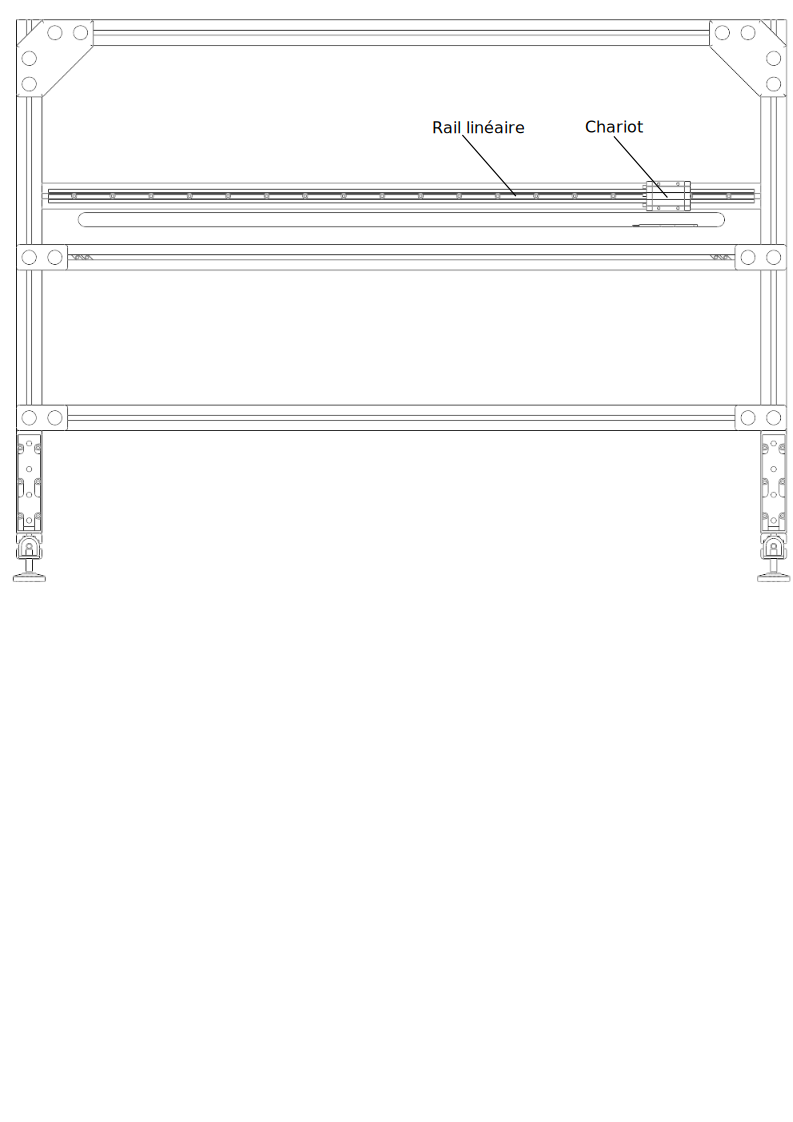
\includegraphics[width = \textwidth]{assets/figures/VueFace.svg}
  \caption{Représentation de la structure en 3D de face avec l'ajout des éléments des solutions}
  \label{fig:VueFace}
\end{figure}

\begin{figure}[H]
  \centering
  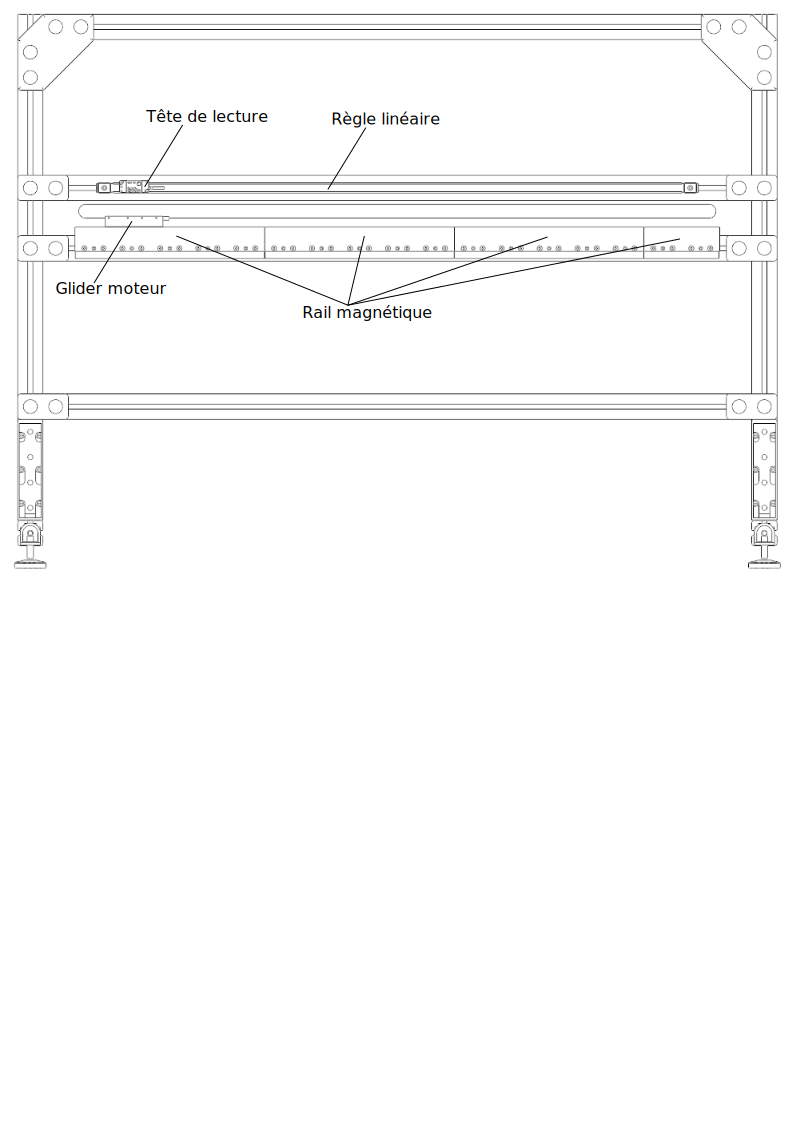
\includegraphics[width = \textwidth]{assets/figures/VueDerriere.svg}
  \caption{Représentation de la structure en 3D de derrière avec l'ajout des éléments des solutions}
  \label{fig:VueDerriere}
\end{figure}

\section{Autres éléments}\label{sec:AutreEle}
D'autres éléments sont encore nécessaires au bon fonctionnement du système.

\subsection{Capteurs de fins de course}
Des capteurs de fins de course sont importants non seulement pour détecter le chariot lorsqu'il s'approche d'un bord, mais aussi
pour faire la mise à zéro au démarrage du système. Dans le cadre de ce projet des capteurs de proximité à contact Reed ont été choisis.
Le choix s'est porté sur le capteur MC-38 de chez Synacorp \cite{Synacorp}. Ce capteur est déjà disponible dans le stock de la \acrshort{Heig}
et possède une résistance en dessous du Ohm lorsqu'un aimant se trouve devant. De plus, ce type de capteur possède une bande adhésive qui lui
permet de se fixer en se collant.

\subsection{Amortisseurs}
Il y a aussi besoin d'amortisseurs en bout de course au cas où le chariot arriverait trop vite pour s'arrêter. Les facteurs clés pour le choix
de ces pièces sont la vitesse maximale qu'elles peuvent amortir et la quantité d'énergie absorbable. Des amortisseurs RB1007 taille M10
de SMC \cite{SMC} ont été choisis à cette fin car ils peuvent tenir une vitesse d'impact de 5~m/s.

\subsection{Chaîne porte-câbles}
Une chaîne porte-câbles pour guider les câbles qui doivent bouger avec le système. Igus \cite{Igus} possède une grande variété de choix dans
ce domaine-là. Le choix s'est porté sur la chaîne System E2 mini Série 14 d'une longueur de 1220~mm avec des éléments de fixations.

\subsection{Encodeur de position angulaire}
L'encodeur de position angulaire permet de déterminer l'angle auquel se trouve la tige. Le stock de la \acrshort{Heig} possède déjà un encodeur
utilisable, il s'agit de l'encodeur TMCS-20 de Trinamic \cite{Trinamic}. Il possède une résolution de 32768 incréments ce qui est capital car
plus la résolution sur l'angle de la tige est bonne plus la régulation du système sera facile.